
\documentclass[11pt,a4paper]{article}
\usepackage[left=2cm,right=2cm,top=2cm,bottom=3cm]{geometry}
\usepackage{amsmath,amsfonts,amsthm,amssymb,varioref,times, commath}
\usepackage{gensymb}
\usepackage{tikz}
\usepackage{textcomp}
\usepackage{hyperref}
\hypersetup{
 colorlinks=true,
 linkcolor=blue,
 filecolor=magenta, 
urlcolor=cyan,
}
\usepackage{lipsum}
\usepackage{epigraph}
%to resume numbering in a list
\usepackage{enumitem}
%----- arrows 
\usepackage{extarrows}

%    differential equatiosn 
\usepackage{diffcoeff}   %\diff[2]{x}{y}


%%%%%%pour ecrire en français avec les accents
\usepackage[utf8]{inputenc}
\usepackage[T1]{fontenc}
\usepackage{lmodern} % load a font with all the characters
\usepackage{units}
%%%%%%%Image-related packages
\usepackage{wrapfig}
\usepackage{float, graphicx}
\graphicspath{ {./img/} }
\usepackage{subcaption}
\usepackage[export]{adjustbox}

%%%%%%%pour faire des cadres
\usepackage{xcolor}
\usepackage{tcolorbox}
\usepackage{framed}
\usepackage{mdframed}


%%%%%%%chemistry frmulae
\usepackage{chemfig}
\usepackage{chemformula}
\usepackage[version=4]{mhchem}

% -------------- Circuits -------------------
\usepackage[european, straightvoltages]{circuitikz}

% Title & headers
\usepackage[explicit]{titlesec}
% Raised Rule Command:
% Arg 1 (Optional) - How high to raise the rule
% Arg 2 - Thickness of the rule
\newcommand{\raisedrulefill}[2][0ex]{\leaders\hbox{\rule[#1]{1pt}{#2}}\hfill}
\titleformat{\section}{\Large\bfseries}{\thesection. }{0em}{#1\,\raisedrulefill[0.4ex]{1pt}}

% pour ecrire sur +sieurs colonnes
\usepackage{multicol}
\setlength{\columnseprule}{0pt}
\setlength{\columnsep}{60pt}
% Fusion de lignes de tableaux.
\usepackage{multirow}
% Position verticale des lettres dans la ligne de tableau.
\usepackage{array}

% physics -----------------------------------------------------------
\newcommand{\To}{\longrightarrow}
\newcommand{\gpl}{\; g\cdot L^{-1}}
\newcommand{\gpmol}{\; g\cdot mol^{-1}}
\newcommand{\mpl}{\; mol\cdot L^{-1}}
\newcommand{\mps}{\; m\cdot s^{-1}}
\newcommand{\rps}{\; rad\cdot s^{-1}}
\newcommand{\kph}{\; km\cdot h^{-1}}
\newcommand{\mpss}{\; m\cdot s^{-2}}
\newcommand{\Dt}{\Delta t}
\newcommand{\vv}{\vec{v}}
\newcommand{\va}{\vec{a}}
\newcommand{\vp}{\vec{p}}
\newcommand{\vf}{\vec{F}}
\newcommand*{\Vf}[1]{\overrightarrow{F_\ensuremath{{#1}}}}
\newcommand{\es}[1]{\cdot10^{#1}}
\newcommand{\eng}[1]{\textcolor{purple}{(= #1})}
\usepackage{harpoon}
%\newcommand*{\vect}[1]{\overrightharp{\ensuremath{#1}}}
\newcommand*{\Vect}[1]{\overrightarrow{\ensuremath{#1}}}
\newcommand{\pfd}[1]{\sum \vec{F}_{ext_{#1}} &= \od{\vp_{#1}}{t} = m\cdot\va_{#1}}
\newcommand{\C}{\degree C}
\newcommand{\Delt}{\Delta t}

% --- Circuits ------------
\newcommand{\bipole}[1]{
\begin{circuitikz} \draw
(0,0) to[ #1 ] (2,0); 
\end{circuitikz} {\hspace{5mm}}}

% Chimie ---------------------------------
\newcommand{\oxo}{\ce{H3O+}_{(aq)}}
\newcommand{\eau}{\ce{H2O}_{(\ell)}}
\newcommand{\OH}{\ce{HO-}_{(aq)}}
\newcommand{\AH}{\ce{AH}_{(aq)}}
\newcommand{\A}{\ce{A-}_{(aq)}}
\newcommand{\MnO}{\ce{MnO_4^{-}}}
\newcommand{\conc}[1]{\left[{#1}\right]}
\newcommand{\couple}[2]{\ce{#1/#2}}


% Environnements ------------------------
\newcounter{exo}
\newenvironment{exo}[1][]
{\refstepcounter{exo} \begin{shaded}\noindent $\triangleright \quad$\textbf{Exercice~\theexo. #1} } { \end{shaded}}
\newenvironment{eg}
{\begin{shaded} \textbf{Exemple:} } { \end{shaded}}

\newenvironment{defn}[1]
{\begin{leftbar}\noindent \textbf{Définition :\textit{ \quad #1}} } { \end{leftbar}}

%\newenvironment{rmrq}
%{\begin{shaded} \textbf{Remarque.\quad } \itshape } { \end{shaded}}
\newenvironment{rmrq}
{\begin{mdframed}[backgroundcolor=blue!10, linewidth=0pt] \textbf{Remarque.\quad } \itshape } { \end{mdframed}}

\newenvironment{python}
{\begin{shaded} \textbf{A faire en PYTHON}\\ \itshape } { \end{shaded}}

% Shading colour -----------------------------
\definecolor{shadecolor}{gray}{0.9}

\date{}
\author{}

\renewcommand*\contentsname{Résumé}









% Title & headers 
\usepackage{fancyhdr}
\pagestyle{fancy}
\fancyhf{}
\lhead{SciPhy : Terminale spé}
\rhead{$\Phi $ - 2 : Mécanique Newtonienne}
\chead{2020-28}
\rfoot{Page \thepage}
\lfoot{\textcopyright\; S Zayyani}
\renewcommand{\footrulewidth}{0.1pt}% default is 0pt


\title{\large Physique - Chapitre 2 \\ \LARGE  La mécanique newtonienne : Les lois de Newton \\}

\date{}
\author{}

\setlength{\parindent}{0mm}
\setlength{\parskip}{2mm}

%%%%%%%%%%% For wrapfigure 
\setlength{\intextsep}{1pt}%
\setlength{\columnsep}{4pt}%

\begin{document}
\maketitle

\vspace{-1cm}

\begin{tcolorbox}[title=Notions de la classe de première à rappeler]
calcul d'une dérivée ; principe d'inertie ; vecteurs ; trigonométrie ; décompositions des forces
%\tcblower
\end{tcolorbox}
\tableofcontents

\section{Un peu d'histoire}

La mécanique newtonienne, qui aujourd'hui porte plutôt l'appellation "mécanique classique" \eng{classical mechanics} est un domaine vaste est important de la physique. La mécanique peut être catégorisé selon la nature de l'objet étudié (mécanique du point, mécanique du solide, mécanique des fluides, etc). Mais le lus souvent elle est souvent sous catégorisée en
\begin{itemize}
    \item \textbf{Cinématique \eng{kinematics} : }l'étude (et la description) du mouvement independamment de ses causes
    \item \textbf{Statique \eng{statics} : }l'étude des objects en équilibre (immobile ou en mouvement rectiligne uniforme)
    \item \textbf{Dynamique \eng{dynamics} : }l'étude des causes du mouvement des objects
\end{itemize}

Le scientifique le plus responsable pour la "création" de la mécanique est Galilée au $XIV^e$ siècle (même si il y a eu des penseurs même antiques, comme Archimède, qui se sont penchés sur des questions du mouvement), mais c'est Newton qui formalise, approfondi et transforme la mécanique un en outil mathématique et très puissant calculatoire. La mécanique a longtemps était traité comme un domaine des mathématiques, jusqu'à Newton, et même après de nombreux contributions importantes ont été faites, souvent par des mathématiciens (e.g. Lagrange, Hamilton, Laplace ... ) et à nos jours reste un des domaines de la physique le lus mathématiques et plus développé dans sa description mathématique. 

Cette année nous nous limitons aux lois de Newton, qui malgré leur simplicité, ont eu des applications innombrables (c.f. aller sur la Lune!). Elles se résument : 
\begin{itemize}
    \item $1^{ère}$ loi : Principe d'inertie
    \item $2^{ème}$ loi : Principe fondamental de dynamique
    \item $3^{ème}$ loi : Principe des actions réciproques
\end{itemize}

Il est important de noter qu'en Terminale nous nous limitons aux mouvement exclusivement dans des référentiels galiléens. Allez, c'est parti! 

\section{Quantité de mouvement}

\begin{defn}{Quantité de mouvement \eng{Momentum}}
\begin{itemize}
    \item la quantité de mouvement, noté $\Vec{p}$ est une \textbf{grandeur vectorielle} associée au vecteur-vitesse, et à la masse d'un corps. 
    \item la quantité de mouvement est le \textbf{produit de la masse et du vecteur vitesse} : 
    \[ \Vec{p} = m\cdot\vv \]
    \item la quantité de mouvement s'exprime en $kg\cdot m\cdot s^{-1}$. 
\end{itemize}
\end{defn}

\begingroup
\setlength{\columnsep}{15pt}%
\begin{wraptable}{l}{0.3\linewidth}
\begin{rmrq}
\small{La quantité de mouvement est souvent la grandeur préférée pour la caractérisation d’un mouvement, car elle inclue la masse aussi, ce qui devient important quand on verra la relativité restreinte d’Einstein. 

En fait, la quantité de mouvement est une des propriétés fondamentales d'un corps en mouvement, plus fondamentale encore que son vecteur-vitesse. Nous parlons donc souvent de la modification ou de la variation de la quantité de mouvement. }
\end{rmrq}
\end{wraptable}

Comme c'est souvent le cas, on essaie de donner un sens au comportement d'un corps quand certaines caractéristiques varient, ou sont conservées. 

Voyons le sens de la conservation de la quantité de mouvement dans le temps. Conservation dans le temps, mathématiquement, correspond à une variation nulle dans le temps, autrement dit, la dérivée d'une grandeur conservée dans le temps est nulle par rapport à la variable du temps : 
\[
\od{\vp}{t} = \Vec{0} \quad \Longleftrightarrow\quad \vp = \text{const}
\]
Autrement dit, dans le cas de la conservation de la quantité de mouvement $m\cdot\vv = \Vec{0}$ et la masse étant constante (dans notre cas) $ \vv = \Vec{0}$. 

Quand la quantité de mouvement est conservée le vecteur-vitesse reste inchangé, et le mouvement est donc rectiligne et uniforme, et vice versa. 

\endgroup

En revanche, dans le cas ou la quantité de mouvement n'est pas conservée, 
\[
\od{\vp}{t} \ne \Vec{0} \quad \Longleftrightarrow\quad \vp \ne \text{const}
\]
Le mouvement n'est donc pas rectiligne uniforme, c'est à dire quand la quantité de mouvement n'est pas conservée le mouvement est accéléré, et l'inverse, un mouvement accéléré n'est conserve la quantité de mouvement. 

Revenons à cette de la quantité de mouvement et creusons un peu plus, en appuyant sur la définition de cette grandeur : 
\[ \od{\vp}{t} = \od{}{t}(m\cdot\vv) = m\cdot\od{\vv}{t} = m\cdot\va \]
Ce que l'on voit sera éclairci dans les parties suivante, mais une coup d'\oe il rapide nous révèle un lien entre la quantité de mouvement et l'accélération du corps, un lien fondamental, établit, comme nous verrons très rapidement par l'action des forces extérieures sur le corps. 

\begin{exo}
Calculer la quantité de mouvement d’une voiture, ayant une masse de $800\; kg$, qui roule à $50\kph$. 
\vspace{2.5cm}
\end{exo}

\begin{exo}
Un camion ayant une masse de  $10\; tonnes$, roule à $108\kph $. 

A quelle vitesse doit rouler une voiture ayant une masse de $1200\; kg$, pour avoir la même quantité de mouvement ? Et pour avoir la même énergie cinétique ? 
\vspace{3cm}
\end{exo}

\subsection{Conservation de la quantité de mouvement}

Dans certaines conditions, notamment en absence de forces extérieures, ou l'annulation des forces extérieures, la quantité de mouvement d'un corps se conserve.  Mais d'abord une définition très importante.

\begin{defn}{Système pseudo-isolé}
\begin{itemize}
    \item Un système mécanique est considéré comme \textbf{isolé} s'il ne subit aucune force extérieure. 
    \item Un système mécanique est considéré comme \textbf{pseudo-isolé} s'il la somme des forces extérieure agissant sur lui est nulle. 
    \item En mécanique de Newton, un système isolé et pseudo-isolé sont équivalents. 
\end{itemize}
\end{defn}

L'énoncé, donc, du principe de la Conservation de la quantité de mouvement est 
\begin{shaded}
\textbf{La quantité de mouvement totale d'un système isolé ou pseudo-isolé est conservée dans le temps.} 
\end{shaded}
Ce principe s'applique à un système composé d'un seul corps, autant qu'à un système composé de plusieurs corps différents. Il n'y a aucune différence dans l'application. La seule différence étant que dans le cas d'un système multi-corps c'est la somme des quantité de mouvement qui reste inchangé même si le mouvement de chaque corps individuel peut varier. 

De manière générale, comme nous allons voir une fois passé à l'application du principe, nous calculons la quantité de mouvement du système avant et après un certain événement, comme une collision. 

\begin{eg}
Deux patineurs $1$ et $2$ de masses $m_1 = 50\; kg$ et $m_2 = 85\; kg $ sont immobiles et côte à côte en face, sur un patinoire horizontale. A l'instant $t_1$ ils se repoussent mutuellement, et par conséquent commencent à s'éloigner l'un de l'autre. Si $v_1 = 5,0\mps$, déterminer la vitesse $v_2$. 

\textbf{Solution : }


\begin{wrapfigure}{r}{0.35\textwidth}
\centering
\tikzset{every picture/.style={line width=0.75pt}} %set default line width to 0.75pt        

\begin{tikzpicture}[x=0.75pt,y=0.75pt,yscale=-1,xscale=1]
%uncomment if require: \path (0,300); %set diagram left start at 0, and has height of 300

%Straight Lines [id:da004905175420697683] 
\draw    (100,128) -- (235.5,128) ;
%Straight Lines [id:da876797870477527] 
\draw    (161,127) -- (161,185) ;
\draw [shift={(161,187)}, rotate = 270] [color={rgb, 255:red, 0; green, 0; blue, 0 }  ][line width=0.75]    (10.93,-3.29) .. controls (6.95,-1.4) and (3.31,-0.3) .. (0,0) .. controls (3.31,0.3) and (6.95,1.4) .. (10.93,3.29)   ;
%Straight Lines [id:da13808569470402254] 
\draw    (161,127) -- (161,73.43) ;
\draw [shift={(161,71.43)}, rotate = 450] [color={rgb, 255:red, 0; green, 0; blue, 0 }  ][line width=0.75]    (10.93,-3.29) .. controls (6.95,-1.4) and (3.31,-0.3) .. (0,0) .. controls (3.31,0.3) and (6.95,1.4) .. (10.93,3.29)   ;

% Text Node
\draw (163,190.4) node [anchor=north west][inner sep=0.75pt]    {$F_{g}$};
% Text Node
\draw (160.96,50.88) node [anchor=north west][inner sep=0.75pt]  [rotate=-359.71]  {$F_{N}$};
\end{tikzpicture}
\end{wrapfigure}

Il faut d'abord identifier notre système d'étude. Ici le système est $\{ 1 + 2 \} $, l'ensemble des deux patineurs. 

En suite, il faut déterminer ou s'assurer que le système choisi est bien (pseduo-)isolé, car sinon le système ne conserve pas sa quantité de mouvement. Ceci nécessité un diagramme de bilan des forces (ci-contre).

Le fait que les deux soit sur la glace, nous permet l'approximation de l'absence de toute force de frottement, et donc les seules forces restantes sont la force gravitation $F_g$, et la force normale (réaction du sol) $F_N$; et étant donné que leurs mouvement est purement horizontal, et rectiligne et uniforme, ces deux forces s'annulent. Et donc la somme de toutes les forces est nulle, ce qui nous permet de dire que le système est bien pseudo-isolé. 

On peut maintenant dire que la quantité de mouvement du système se conserve, et plus précisément, la quantité de mouvement des deux patineurs, avant qu'ils se poussent, est la même qu'après (souvent dénoté par l'ajout d'un " ' (prime) " : \begin{align*}
    \vp_{système} &= \vp_{système}' \\
    \vp_1 + \vp_2 &= \vp_1' + \vp_2'\\
    m_1\vv_1 + m_2\vv_2 &= m_1\vv_1' + m_2\vv_2' 
\end{align*} 
Il faut maintenant passer de la notation vectorielle en notation algébrique et donc on dénote le sens du mouvement par des signes $+/-$. 

Les deux patineurs sont immobiles au-début, et donc le système possède une quantité de mouvement nulle pour commencer. Cette grandeur est conservée, et donc cette somme doit rester nulle même après, quand chaque composante du système aura une quantité de mouvement non-nulle, dont le signe dépend du sens du mouvement dans la direction horizontale (le choix de signe pour chaque sens est un choix arbitraire). 
\begin{align*}
    m_1v_1 + m_2v_2 &= m_1v_1' + m_2v_2' \\
    0 + 0 &= m_1v_1' + m_2v_2' \\
    m_1v_1' &= - m_2v_2' \\
    v_2 &= -\dfrac{m_1}{m_2}v_1
\end{align*} 
Sans faire un calcul numérique on peut déjà apprendre quelques chose de la nature du mouvement du deuxième patineur : il se déplace dans le sens opposé au premier patineur. Oui, c'est parfaitement logique, mais c'est toujours mieux quand le calcul théorique confirme une évidence telle. Passons à l'application numérique : 
\begin{align*}
    v_2 &= -\dfrac{m_1}{m_2}v_1 \\
    v_2 &= -\dfrac{85}{50}(5,0) \\
    v_2 &= -8,5\mps
\end{align*} 
Le deuxième patineur se déplace donc avec une vitesse de $8,5\mps$ dans le sens opposé à son partenaire. 
\end{eg}

\section{$1^{ère}$ loi : Principe d'inertie}%%%%----------------SECTION

\begin{quote}
    \centering
    \small{« Lex I : Corpus omne perseverare in statu suo quiescendi vel movendi uniformiter in directum, nisi quatenus a viribus impressis cogitur statum illum mutare »}
    
    \small{« Loi I : Tout corps persévère dans l'état de repos ou de mouvement uniforme en ligne droite dans lequel il se trouve, à moins que quelque force n'agisse sur lui, et ne le contraigne à changer d'état. »}
\end{quote}

Nous connaissons déjà cette loi, car vous l'avez étudiée (abondamment et en détail) en classe de $2^{onde}$, mais - comme d'habitude - on vous a raconté seuelement un parite de l'histoire. Comblons donc cette lacune: Le principe d’inertie (la première loi) \textit{n’est valable que dans certains référentiels.} Par exemple, un raisonnement selon ce principe, ne donnera pas la bonne conclusion dans les cas suivant :
\begin{itemize}
    \item Une personne assise dans une voiture qui accélère vers l’avant
    \item Des enfants sur un manège en mouvement
    \item Un objet en chute libre
\end{itemize}

Les référentiels dans lesquels on peut appliquer le principe d’inertie sont des référentiels dits Galiléen (ou inertiels).  

Donc nous pouvons énoncer cette loi dans un langage plus moderne : 
\begin{quote}
« Dans un référentiel galiléen, le vecteur-vitesse du centre d'inertie d'un système est constant si et seulement si la somme des vecteurs forces qui s'exercent sur le système est un vecteur nul.»
\end{quote}

En reformulant cette loi en langage (plus moderne) de la quantité de mouvement 

\begin{shaded}
\textbf{« Dans un référentiel galiléen, si la résultante de toutes les forces est un vecteur-nul, le corps conserve sa quantité de mouvement ». }
\end{shaded}

\section{$2^{ème}$ loi : Principe fondamental de dynamique}%%%%----------------SECTION

\begin{quote}
    \centering
    \small{« Lex II : Impressae de motrici de l'esse vi de proportionalem de motus de Mutationem et imprimitur d'illa de force de qua de rectam de lineam de secundum de fieri.»}
    
    \small{« Loi II : L'altération du mouvement est proportionnelle à la force qui lui est imprimée ; et cette altération se fait en ligne droite dans la direction de la force. »}
\end{quote}

La deuxième loi de Newton est une extension naturelle de la première loi, elle concerne le comportement d’un corps quand, justement, la somme vectorielle des forces extérieures n’est pas nulle.  Selon le principe d’inertie, si la somme des forces n’est pas nulle, alors le mouvement \textit{n’est plus} rectiligne uniforme (ou repos).  Quel serait-elle alors sa nature ?

La deuxième loi de Newton s’énonce ainsi, dans un langage moderne :
\begin{quote}
«Dans un référentiel galiléen, la variation du vecteur-vitesse (i.e. accélération) est proportionnelle à la somme des forces qui s’exercent sur le corps. »
\end{quote}

Ou, autrement dit 
\[
\sum \vec{F}_{ext} \propto \Vect{\Delta v_G}
\]
et donc, en remplaçant la propotionnalité par une égalité, on introduit la constante de proportionnalité $m$, 
\[
\sum \vec{F}_{ext} = m\cdot\Vect{a_G}
\]

Pour un objet en mouvement rectiligne uniforme $\Vect{\Delta v_G}=\Vec{0}$ (et donc l’accélération $\va$). Par conséquent, si $\Vect{\Delta v_G}\ne\Vec{0}$, on en conclue que le système subit des forces extérieures qui ne se compensent pas.  De plus, si l'on connaît la direction et le sens de $\Vect{\Delta v_G}$ , on en déduit la direction et le sens de la somme des forces extérieures.  

Selon Newton, ce n’est donc pas la valeur (absolue) de la vitesse qui est liée aux forces agissant sur le corps, mais plutôt la variation de la vitesse.  C'est à dire qu'un objet en mouvement rectiligne uniforme avec une très grande vitesse est exactement comme un objet en mouvement rectiligne uniforme avec une vitesse très faible, car dans les deux cas, les corps ne subissent aucune force (ou la somme des forces est nulle), et le vecteur-vitesse du système reste inchangé. 

Ayant établi la caractéristique fondamentale de la quantité de mouvement, exprimons le principe fondamental de la dynamique (PFD) en ces termes 
\[
\sum \vec{F}_{ext} = m\cdot\va = m\cdot\od{\vv}{t} = \od{m\cdot\vv}{t}
\]
\begin{shaded}
Et nous avons donc l'expression plus moderne du PFD : 
\[
\sum \vec{F}_{ext} = \od{\vp}{t}
\]
Et en trois dimensions : 
\begin{align*}
   \sum \vec{F}_x &= \od{\vp_x}{t} = m\cdot\od{\vv_x}{t} = m\cdot\va_x \\
   \sum \vec{F}_y &= \od{\vp_y}{t} = m\cdot\od{\vv_y}{t} = m\cdot\va_y \\
   \sum \vec{F}_z &= \od{\vp_z}{t} = m\cdot\od{\vv_z}{t} = m\cdot\va_z 
\end{align*}
\end{shaded}
C’est-à-dire que toute variation de la quantité de mouvement est due aux forces extérieures non-compensées, ou autrement dit, si la résultante des forces extérieures n’est pas un vecteur-nulle, la conséquence est une variation de la quantité de mouvement.  


Il est, néanmoins, important de noter que cette relation $(\sum \vec{F}_{ext} = \od{\vp}{t})$ est \textit{plus générale} que celle d’avant, et en fait se simplifie à la relation précédente que l’on connaît bien $(\sum \vec{F}_{ext} = m\cdot\va$) seulement dans le cas où la masse est constante. Ceci devient important dans quelques cas, comme par exemple : 

\begingroup
\setlength{\columnsep}{15pt}%
\setlength{\intextsep}{-10pt}%
\begin{wraptable}{r}{0.4\linewidth}
\begin{rmrq}
\small{ \emph{Si l’on peut donc montrer que le principe d’inertie est simplement un cas particulier de la deuxième loi, pourquoi l’énoncer comme une loi à part et distincte ? }

Bonne question ! Il est très important de ne pas oublier que cette loi n’est valable que dans un référentiel inertiel. Il ne faut donc justement pas considérer la 1e loi comme un cas particulier de la 2e loi, mais plutôt comme un postulat qui établit la définition d’un référentiel inertiel/galiléen sans lequel il n’est pas possible d’énoncer ou d’établir la deuxième loi.}
\end{rmrq}
\end{wraptable}

\begin{itemize}
    \item Le cas où il y a une perte de masse, comme dans les systèmes qui éjectent de la matière afin de se propulser (l’éjection de la matière est une perte de masse)
    \item le cas d’un mouvement aux vitesses « relativistes », c’est-à-dire des mouvements à de très grandes vitesses (rapprochant la vitesse de la lumière).
    \item dans le cas de mouvement des objets sans une "masse stationnaire" possédant néanmoins une quantité de mouvement.
\end{itemize}

\begin{exo}
Montrer que la première loi (principe d’inertie) n’est qu’un cas particulier de la deuxième loi (i.e. retrouver la première loi à partir de la deuxième loi).  
\vspace{4.9cm}
\end{exo}
	
\endgroup	 

\section{$3^{ème}$ loi : Actions réciproques}
\begin{quote}
    \centering
    \small{« Lex III : Actioni contrariam semper et æqualem esse reactionem: sive corporum duorum actiones in se mutuo semper esse æquales et in partes contrarias dirig »}
    
    \small{« Loi III : « L'action est toujours égale à la réaction ; c'est-à-dire que les actions de deux corps l'un sur l'autre sont toujours égales et de sens contraires. »}
\end{quote}

C’est-à-dire, considérons deux systèmes $A$ et $B$ en interaction.  Soient $\Vect{F_{B/A}}$ la force associée à l’action exercée par $B$ sur $A$, et $\Vect{F_{A/B}}$  la force associée à l’action exercée par A sur B.  Quel que soit l’état de mouvement de $A$ par rapport à $B$, on peut toujours écrire l’égalité vectorielle :  $ \Vect{F_{A/B}} = - \Vect{F_{B/A}}$

Considérons maintenant deux patineuses sur la glace.  Elles commencent à l’instant t=0 immobile, face à face, puis elles se poussent l’une contre l’autre. En les prenant toutes les deux comme le système d’étude,  on peut donc écrire : 
$$ \Vect{F_{A/B}} = - \Vect{F_{B/A}} $$  
Et en appliquant le PFD : 
\[ \od{\vp_B}{t} = -\od{\vp_A}{t} \quad \Leftrightarrow \quad \od{\vp_B}{t} + \od{\vp_A}{t} = \vec{0}\]
Définissant notre système comme $\{ A + B \}$ alors 
\[ \od{( \vp_B + \vp_A )}{t} = \vec{0}  \quad \Leftrightarrow \quad \od{\vp_{sys}}{t} = \vec{0} \]
Il est important de bien comprendre le \textit{sens} de ce dernier résultat : la quantité de mouvement du système se conserve. La conservation de la quantité de mouvement (un principe très important et fondamental de la mécanique) est une conséquence de la 3e loi de Newton (ou plus précisément c’est le principe des actions réciproques qui est une conséquence de la conservation de la quantité de mouvement). 

La troisième loi de Newton donc, dans sa formulation plus moderne devient : 
\begin{shaded}
\textbf{« Dans un référentiel galiléen, si la résultante de toutes les forces est un vecteur-nul, le corps conserve sa quantité de mouvement ». }
\end{shaded}

\begin{rmrq}
Nous voyons donc que, dans un référentiel galiléen, la troisième loi de Newton et la conservation de la quantité de mouvement sont intimement liés. Newton pensait que la conservation de la quantité de mouvement était \emph{une conséquence} de sa troisième loi, mais nous considérons aujourd’hui, étant donné que la conservation de la quantité de mouvement est considérée comme un principe plus fondamental, c’est la $3^{ème}$ loi de Newton qui est une conséquence de cette loi de conservation. De cette manière, nous sommes capables d’expliquer des phénomènes divers tels que la propulsion, mouvement des balles de billard, etc. 
\end{rmrq}

\begingroup
\begin{wrapfigure}{r}{0.5\textwidth}
  \centering
  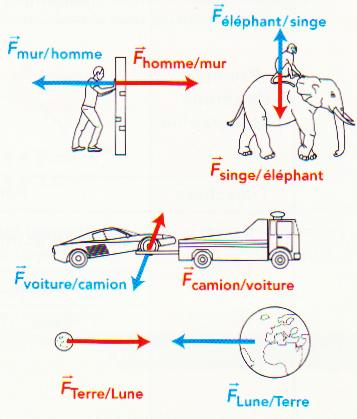
\includegraphics[width=0.95\linewidth]{imgs/p2/acreac.jpg}
  \caption{Quelques exemples des actions réciproques}
\end{wrapfigure}

Voici quelques exemples de ce principe :
\begin{itemize}
    \item Le choc entre un ballon et un mur.  Le ballon exerce une force sur le mur, et le mur réciproquement applique une force sur le ballon. Ce dernier renvoie le ballon, dans le sens opposé.
    \item La terre exerce une force attractive sur la Lune. Réciproquement la Lune applique une force d’une valeur égale mais dans le sens opposé sur la Terre (elle l’attire vers elle-même).
    \item La force exercée par un solide sur son support horizontal est un autre exemple de ce principe.  Un solide placé sur une table subit son poids $\Vf{g}$, qui le tire vers le bas, contre son support, exerçant une force pareille sur ce dernier. Le support à son tour, exerce une force équivalente et dans le sens opposé sur le solide $\vf_{table/solide}$ : c'est la force normale du support.
\end{itemize}
\vfill

\endgroup	

\begin{rmrq}
Les forces $\Vf{A/B}$  et $\Vf{B/A}$  s’exercent sur deux corps différents, on ne peut donc pas dire qu’elles s’annulent ! Deux forces peuvent s’annuler si et seulement si elles agissent sur le même corps ou système (d’où la nécessité de la précision des forces extérieures agissant sur un corps.) 
\end{rmrq}
	
\begin{exo}
    Un avion à hélice peut-il fonctionner dans l’espace ? Pourquoi ? Est-ce pareil pour un missile ?
    \vspace{3cm}
\end{exo}  
	
\begin{exo}
Imaginons que vous êtes devenu un astronaute. Lors des excursions sur la station spatiale vous oubliez de vous attacher à l’extérieure de la station (ahlala !). Pourquoi est-il très dangereux si vous vous détachez du mur de la station ? Pourquoi, dans le cas où vous vous détachez du mur de la station, ne pourriez-vous pas revenir en faisant des mouvements de nage ? Si vous êtes incapable de changer votre mouvement dans l’espace, pourquoi alors une roquette est-elle capable de le faire ? Comment pourriez-vous vous inspirez de ça pour changer votre mouvement dans l’espace ? 
    \vspace{5cm}
\end{exo} 
\vfill
\section{Annexe : Pour aller plus loin ... Chocs élastiques \& inélastiques}

Lors d'une collision entre deux particules, c'est la quantité de mouvement totale du système qui est conservée. Ce principe, de la conservation de la quantité de mouvement, découle directement de la troisième loi de Newton. Dans les exemples qui suivent, nous appliquerons ce principe.

Afin de résoudre ce type de problème, d'abord on s'assure que le système étudié est bien isolé, et puis on applique le principe de la conservation de la quantité de mouvement, et espère qu'il y a assez d'information afin de pouvoir le résoudre. 

Considérons le cas suivant : Une masse $m_1$, ayant une vitesse de $v_1$ selon l'axe $x$, heurte une masse $m2$ initialement immobile. Déterminer les vitesses des deux masses après le choc $v_1'$ et $v_2'$ respectivement. 
\begin{figure}[h]
    \centering
    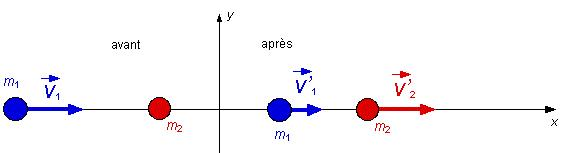
\includegraphics[width=0.8\linewidth]{imgs/p2/choc1.jpg}
\end{figure}
En appliquant le principe de la conservation de la quantité de mouvement nous arrivons à la relation suivante : 
\[   m_1v_1 + m_2v_2 = m_1v_1' + m_2v_2'     \]
Avec $v_1'$ et $v_2'$ inconnus et à déterminer. Une seule équation et deux inconnus. Le seul moyen de résoudre cette équation est de insérer une valeur pour une deux vitesses après le choc et puis calculer l'autre inconnu. Si par exemple nous choisissons une valeur pour $v_1'$, alors 
\begin{align*}
    m_1v_1 + m_2v_2 &= m_1v_1' + m_2v_2' \\
    v_2' &= \dfrac{m_1}{m_2}(v_1 - v_1') + v_2
\end{align*}

Faisons une application et voyons ce que l'on peut apprendre sur le comportement des billes lors d'une telle choc. Prenons les valeurs suivantes : $m_1 = 3\; kg\;,\; m_2=2\; kg\;,\; v_1 = 5\mps \;,\; v_2=0\;,\; v_1'=2\mps$. Après une application numérique on trouve : $v_2' = 4,5\mps $

Calculons maintenant l'énergie cinétique du système avant et après le choc : 
\begin{align*}
    E_{sys} &= E_1 + E_2 = \dfrac{1}{2}m_1v_1^2 + \dfrac{1}{2}m_2v_2^2 \\
    E_{sys}' &= E_1' + E_2' = \dfrac{1}{2}m_1{v_1'}^2 + \dfrac{1}{2}m_2{v_2'}^2 
\end{align*}
Avec les valeur trouvée dans la partie précédente on obtient donc 
\begin{align*}
    E_{sys} &= 37.5\; J \\
    E_{sys}' &= 26.25\; J 
\end{align*}
Ce qui fait une perte de $30 \%$ d'énergie cinétique lors du choc. Mais est-ce toujours le cas? 

Vous pouvez le tester vous-même et vous verrez qu'il y a presque toujours une perte d'énergie, mais pas toujours la même perte. Ce type de choc s'appelle un \textbf{choc inélastique, c'est à dire un choc lors duquel le système perd de l'énergie}, même si la quantité de mouvement est toujours conservée. 

Cette perte peut être due à la déformation des corps, dissipation thermique, dissipation acoustique, etc. Le cas le plus extrême est quand après le choc les deux corps restent collés (imaginez deux voitures après collisions qui restent intriquées), et dans ça cas-là on dit que le choc est \textbf{parfaitement inélastique}. 

Naturellement, il existe une catégories de chocs, où il n'y a pas perte d'énergie appelée des \textbf{chocs élastiques}. Ce sont des chocs pendant lesquels la quantité de mouvement \textbf{ET} l'énergie cinétique du système sont conservées. 

Voilà donc à quoi ressemblent les équations d'un choc élastiques 
\begin{align*}
    p_{sys} &= p_{sys}' \\
    E_{sys} &= E_{sys}' 
\end{align*}
et explicitement 
\begin{align*}
    m_1v_1 + m_2v_2 &= m_1v_1' + m_2v_2'\\
    \dfrac{1}{2}m_1v_1^2 + \dfrac{1}{2}m_2v_2^2  &= \dfrac{1}{2}m_1{v_1'}^2 + \dfrac{1}{2}m_2{v_2'}^2 
\end{align*}
Pour les chocs élastiques nous avons donc un système de deux équations avec deux inconnus, et donc il existe une solution unique que l'on peut déterminer par calcul! Autrement dit, il n'y qu'une seule condition permettant un choc élastique. 

Pour finir, de premier abord, résoudre un tel système d'équation n'est pas forcément évidente (une polynomiale de premier degré et l'autre de second degré), mais avec un peu de gymnastique algébrique, ce système peut être simplifié à deux équations polynomiale de premier degré. Mais, ça c'est à vous de trouver ! 
\newpage


\section{Exercices Résolus}
\begin{figure}[h]
    \centering
    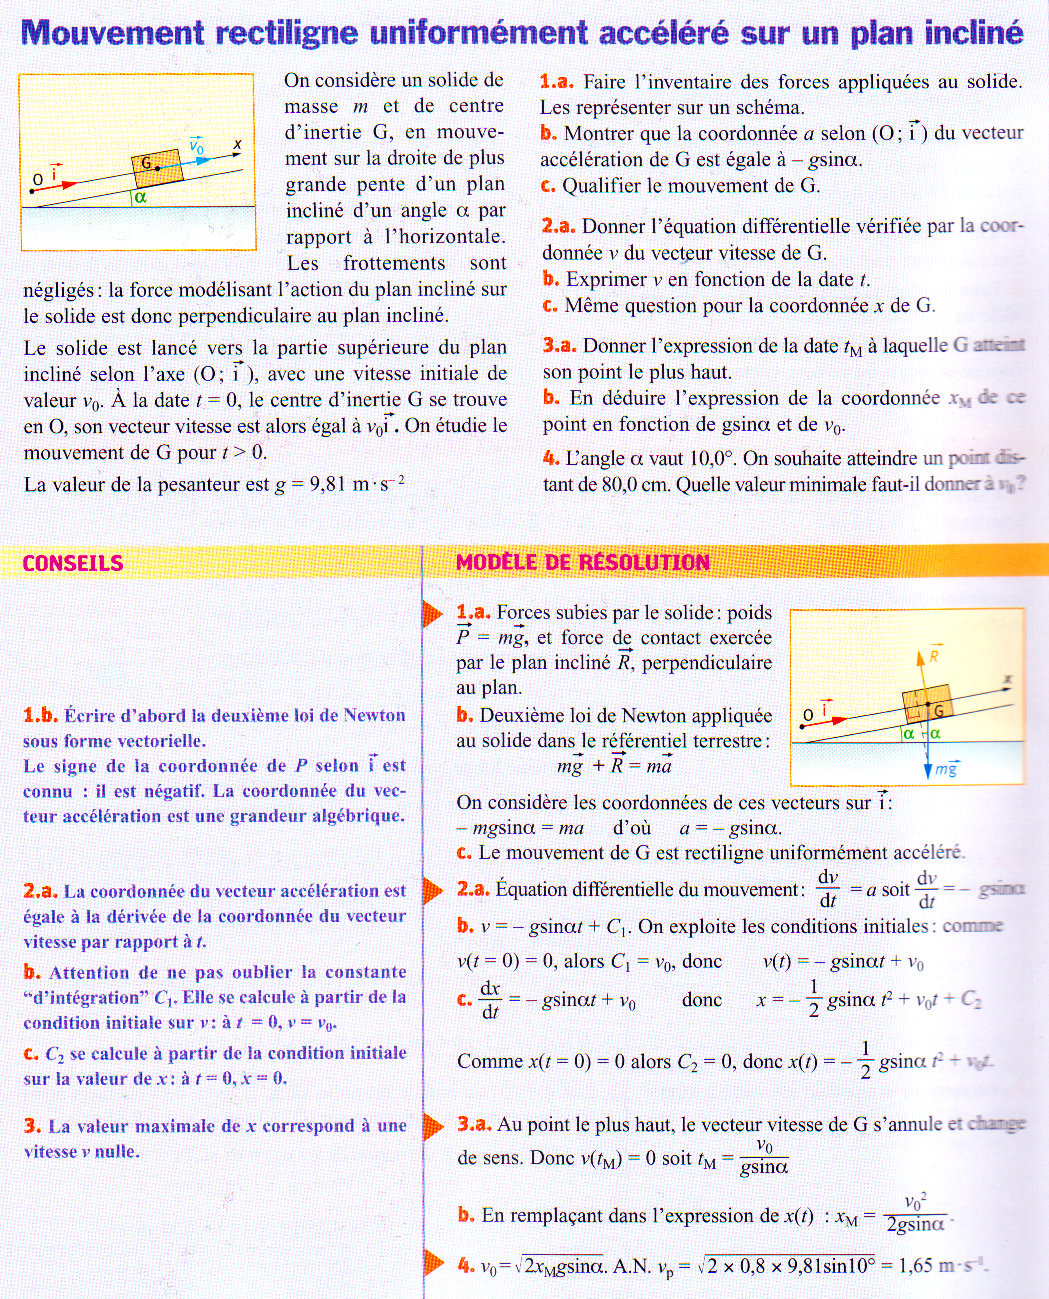
\includegraphics[width=.9\textwidth]{imgs/p2/xo2.jpg}
\end{figure}

\begin{figure}[h]
    \centering
    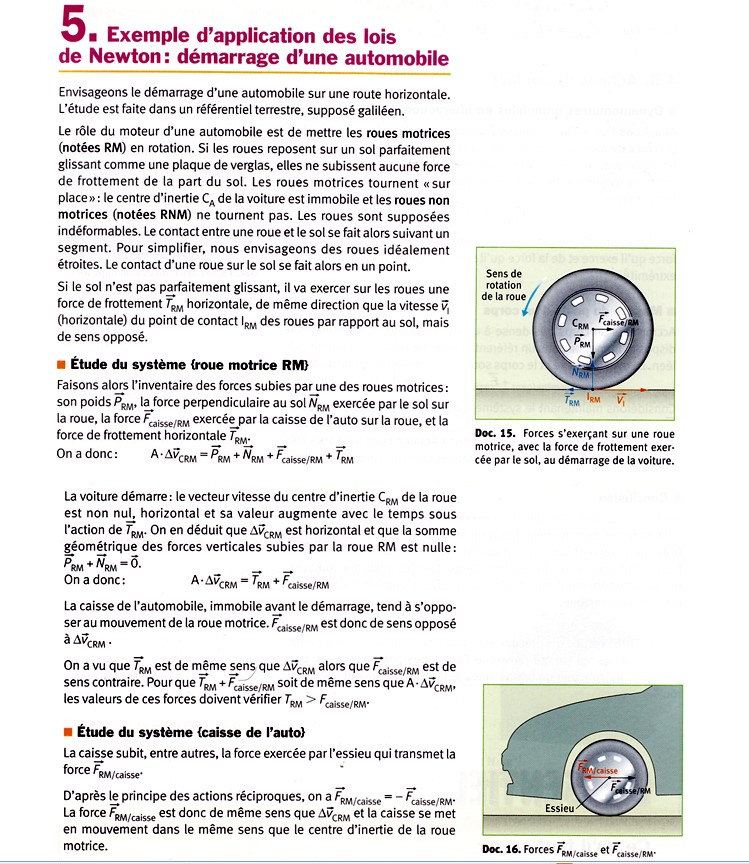
\includegraphics[width=\textwidth]{imgs/p2/xo1.jpg}
\end{figure}

\begin{figure}[h]
    \centering
    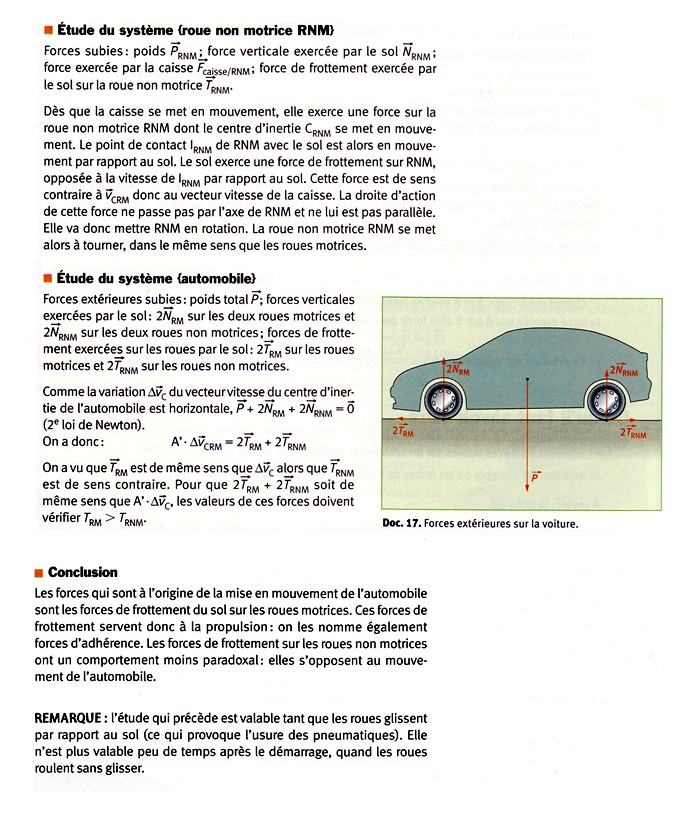
\includegraphics[width=\textwidth]{imgs/p2/xo1b.jpg}
\end{figure}


\end{document}







